\documentclass{article}
\usepackage[a4paper,hmargin={2.4cm,2.4cm},vmargin={2.4cm,2.4cm}]{geometry}
\usepackage[pdftex]{hyperref}
\usepackage{soul}
\usepackage{graphicx}

\begin{document}
\title{Appendix B: BBS Results}
\date{} 
\maketitle
\renewcommand*\thetable{B\arabic{table}}
\renewcommand*\thefigure{B\arabic{figure}}
\begin{table}[htb]
  \centering
  \small
\caption{Model selection table for ovenbirds in Maryland and Virginia,
    1966-2010.  We present model name and number, number of 
parameters (Par.), and difference in Akaike's
information criterion between each model and the top model of
that set ($\Delta$AIC).  The first section compares
models for initial abundance, the second for detection
probability, and the third for dynamics.}
  \begin{tabular}[h]{lcc}
\hline
Model	&Par.	&$\Delta$AIC	\\
\hline
A. Initial Abundance && \\
A.1. NB[$\Lambda$(.)$\alpha$(.)]Exponential[$r$(.)]$p$(.)	&4	&0\\
A.2. P[$\Lambda$(.)]Exponential[$r$(.)]$p$(.)	&3	&1262.7\\
A.3. ZIP[$\Lambda$(.)$\psi$(.)]Exponential[$r$(.)]$p$(.)	&4 &1264.7\\
\hline
B. Detection Probability && \\
B.1. NB[$\Lambda$(.)$\alpha$(.)]Exponential[$r$(.)]$p$(wind+1st)	&8 &0	\\
B.2. NB[$\Lambda$(.)$\alpha$(.)]Exponential[$r$(.)]$p$(wind) &7 &0.9\\
B.3. NB[$\Lambda$(.)$\alpha$(.)]Exponential[$r$(.)]$p$(1st)	&5	&5.0
\\B.4. NB[$\Lambda$(.)$\alpha$(.)]Exponential[$r$(.)]$p$(.)	&4	&6.4\\
\hline
C. Dynamics && \\
C.1. NB[$\Lambda$(.)$\alpha$(.)]Ricker+Immigration[$r$(.)$K$(.)$\iota$(.)]$p$(wind+1st) &10	&0	\\
C.2. NB[$\Lambda$(.)$\alpha$(.)]Gompertz+Immigration[$r$(.)$K$(.)$\iota$(.)]$p$(wind+1st) &10	&8.4 \\
C.3. NB[$\Lambda$(.)$\alpha$(.)]Exponential+Immigration[$r$(.)$\iota$(.)]$p$(wind+1st) &9	&36.5\\
C.4. NB[$\Lambda$(.)$\alpha$(.)]Geometric-recruitment+Immigration[$\gamma$(.)$\omega$(.)$\iota$(.)]$p$(wind+1st) &10	&38.6\\
C.5. NB[$\Lambda$(.)$\alpha$(.)]Gompertz[$r$(.)$K$(.)]$p$(wind+1st) &9	&192.8\\
C.6. NB[$\Lambda$(.)$\alpha$(.)]Ricker[$r$(.)$K$(.)]$p$(wind+1st) &9	&195.1\\
C.7. NB[$\Lambda$(.)$\alpha$(.)]Exponential[$r$(.)]$p$(wind+1st)	&8 &271.3\\
C.8. NB[$\Lambda$(.)$\alpha$(.)]Geometric-recruitment[$\gamma$(.)$\omega$(.)]$p$(wind+1st) &9	&273.7\\
C.9. NB[$\Lambda$(.)$\alpha$(.)]Constant-recruitment[$\gamma$(.)$\omega$(.)]$p$(wind+1st) &9	&1856.7\\
\hline
\end{tabular}
\end{table}
\clearpage

\clearpage
\begin{figure}
  \centering
  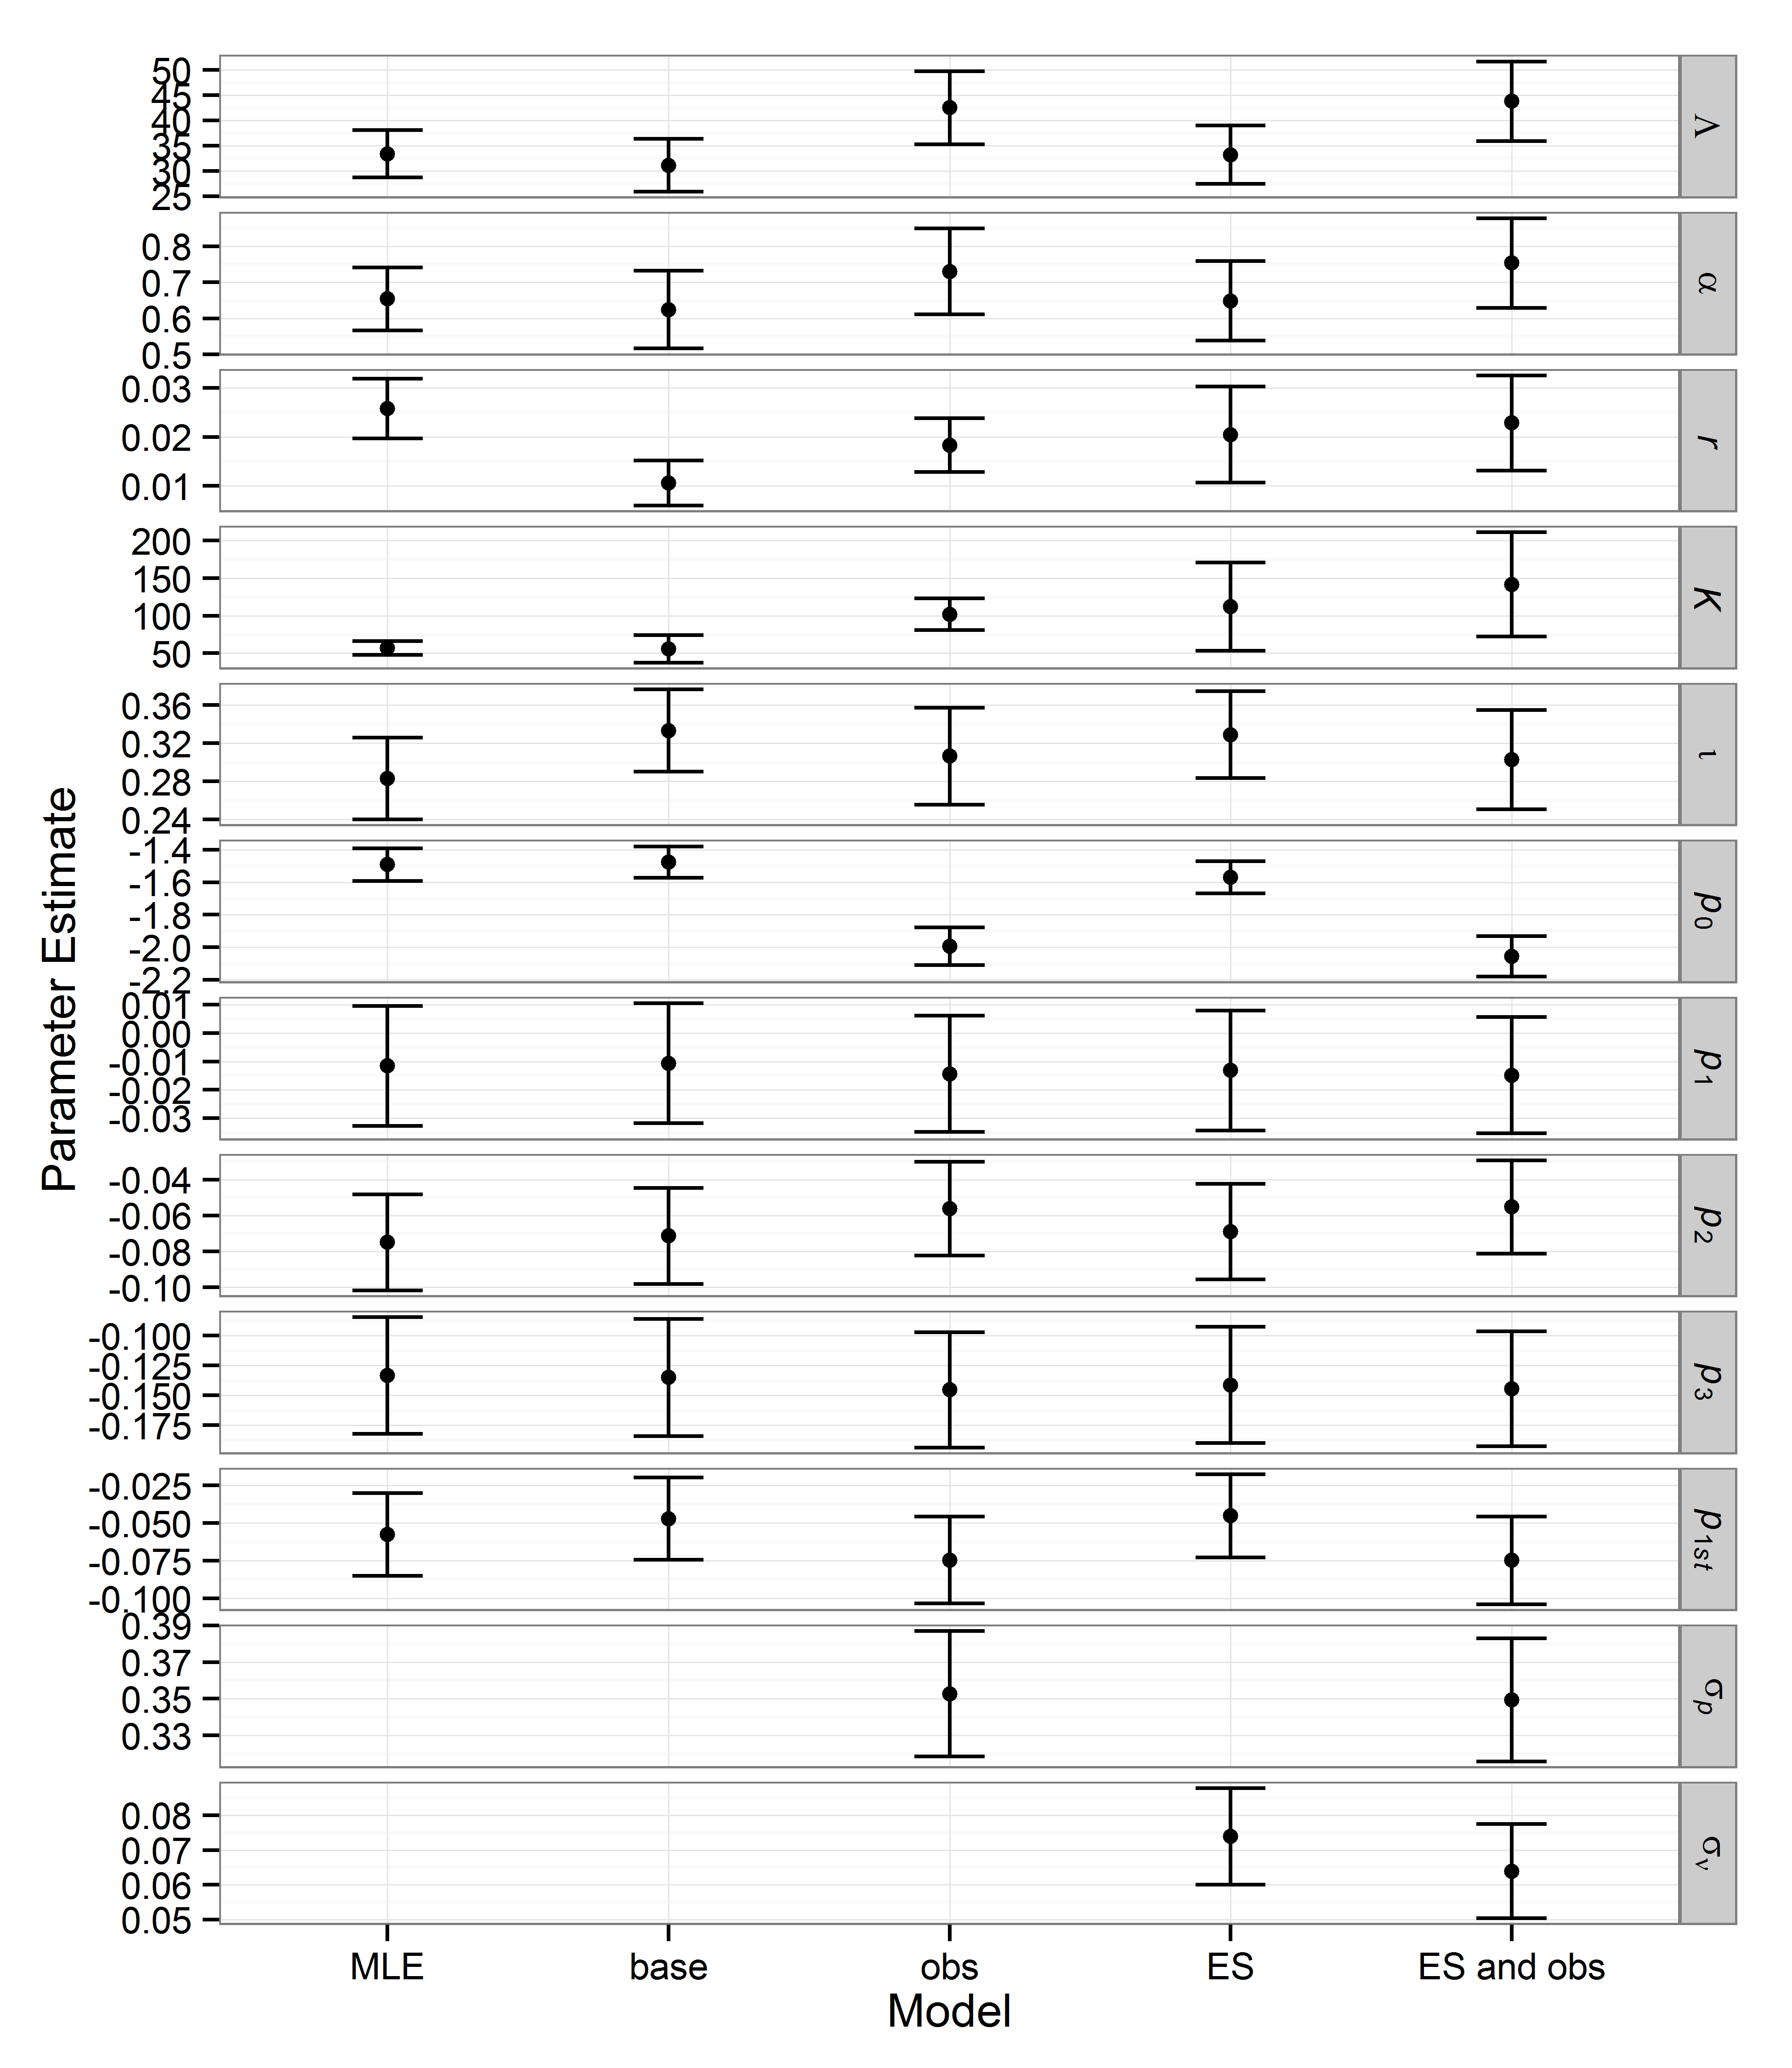
\includegraphics[width=6.5in]{../figs/oven_par_est}
\caption{Parameter estimates for ovenbirds in Maryland and Virginia from BBS data, 1966-2010.  
MLE estimates come from the NB[$\Lambda$(.)$\alpha$(.)]Ricker+Immigration[$r$(.)$K$(.)$\iota$(.)]$p$(wind+1st) 
model run in the \textbf{R} package \texttt{unmarked}; base estimates from the same model run in \textbf{JAGS};
obs estimates from the base model with random observer effects added; and ES estimates from the base
model with regional environmental stochasticity added.  Detectability parameters (intercept: $p_{0}$, 
effect of wind speed 1: $p_{1}$, effect of wind speed 2: $p_{2}$, effect of wind speed 3 or higher: $p_{3}$, 
effect of first run of a route by an observer: $p_{1st}$, and random observer SD: $\sigma_{p}$) are on the 
logit scale. Error bars show SE for MLE estimates and SD for all others.}
\label{fig:oven_par_est}
\end{figure}


\end{document}
